%%%%%%%%%%%%%%%%%%%%%%%%%%%
% Wirtschaftliche Aspekte %
%%%%%%%%%%%%%%%%%%%%%%%%%%%
\section{Wirtschaftliche Aspekte}

\begin{frame}{Kosten und Nutzen I}
    \centering
    Variabler Strompreis (2025-03-06)
    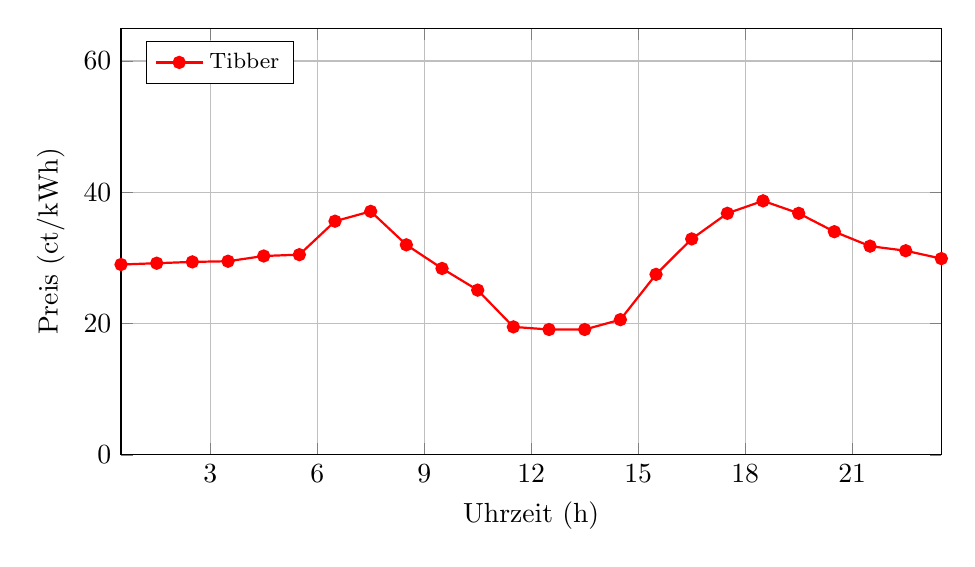
\begin{tikzpicture}
        \begin{axis}[
            width=12cm, height=7cm, % Größe des Plots
            xlabel={Uhrzeit (h)}, % Beschriftung X-Achse
            ylabel={Preis (ct/kWh)}, % Beschriftung Y-Achse
            xtick={0,3,6,9,12,15,18,21,24}, % Markierungen auf der X-Achse
            ymin=0, ymax=65, % Wertebereich für die Preise
            xticklabel style={anchor=north}, % Ausrichtung der X-Achsen-Beschriftung
            yticklabel style={anchor=east}, % Ausrichtung der Y-Achsen-Beschriftung
            grid=major, % Gitterlinien
            enlargelimits=false, % Begrenzung der Achsen direkt an den Rändern
            domain=0:24,
            legend pos=north west,
            legend style={font=\footnotesize},
            legend cell align=left
        ]
        
        \addplot[thick, red, mark=*] coordinates {
            (0.5, 29) (1.5, 29.2) (2.5, 29.4) (3.5, 29.5) 
            (4.5, 30.3) (5.5, 30.5) (6.5, 35.6) (7.5, 37.1) 
            (8.5, 32) (9.5, 28.4) (10.5, 25.1) (11.5, 19.5) 
            (12.5, 19.1) (13.5, 19.1) (14.5, 20.6) (15.5, 27.5) 
            (16.5, 32.9) (17.5, 36.8) (18.5, 38.7) (19.5, 36.8) 
            (20.5, 34) (21.5, 31.8) (22.5, 31.1) (23.5, 29.9) 
        };
        \addlegendentry{Tibber}
        
        % \pgfmathsetmacro{\vntsub}{\vst-\vnt}
        % \pgfmathsetmacro{\vhtadd}{\vht-\vst}

        % %NT:  0.75 ->  0.8925 (netto)
        % %ST:  7.52 ->  9.9488 (netto)
        % %HT: 14.26 -> 16.9694 (netto)
        % \addplot[thick, ForestGreen, mark=triangle, opacity = 0.8] coordinates {
        %     (0.5, 31.17 - \vntsub) (1.5, 30.97- \vntsub) 
        %     (2.5, 30.70- \vntsub) (3.5, 30.65 - \vntsub) 
        %     (4.5, 31.18 - \vntsub) (5.5, 32.19 - \vntsub) 
        %     (6.5, 36.26) (7.5, 38.30) (8.5, 36.72) (9.5, 33.94) (10.5, 31.27)
        %     (11.5, 30.92 + \vhtadd) (12.5, 30.73 + \vhtadd) 
        %     (13.5, 30.95) (14.5, 31.16) (15.5, 33.07) (16.5, 35.97) 
        %     (17.5, 37.75 + \vhtadd) (18.5, 42.83 + \vhtadd) 
        %     (19.5, 40.42) (20.5, 36.68) (21.5, 34.79) 
        %     (22.5, 33.34 - \vntsub) (23.5, 32.14 - \vntsub) 
        % };
        % \addlegendentry{ESTW VNB + Tibber}
        
        \end{axis}
    \end{tikzpicture}
\end{frame}

\begin{frame}{Kosten und Nutzen II}
    Var. Netzentgelte vs. dyn. Strompreis (Übergang 2025-03-12)
    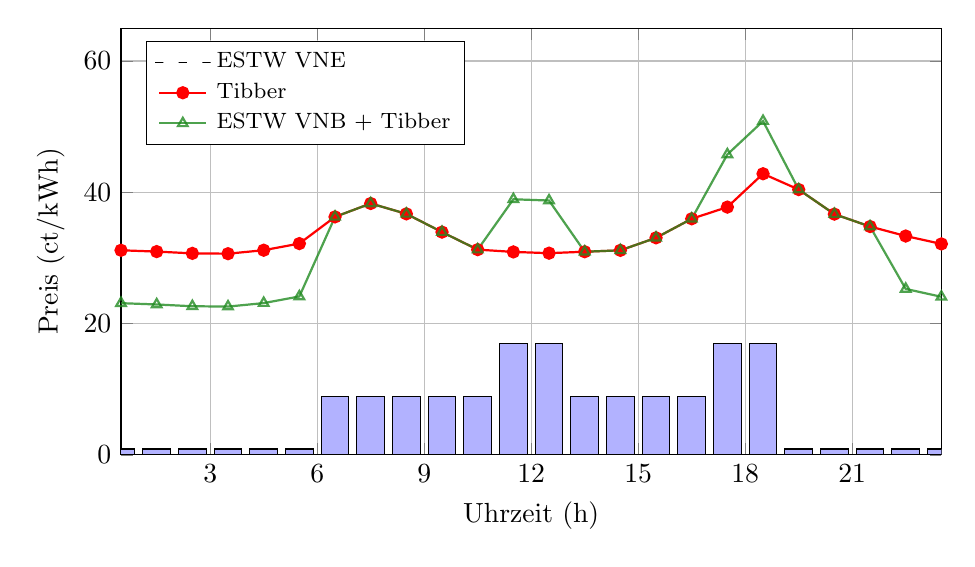
\begin{tikzpicture}
        \begin{axis}[
            width=12cm, height=7cm, % Größe des Plots
            xlabel={Uhrzeit (h)}, % Beschriftung X-Achse
            ylabel={Preis (ct/kWh)}, % Beschriftung Y-Achse
            xtick={0,3,6,9,12,15,18,21,24}, % Markierungen auf der X-Achse
            ymin=0, ymax=65, % Wertebereich für die Preise
            xticklabel style={anchor=north}, % Ausrichtung der X-Achsen-Beschriftung
            yticklabel style={anchor=east}, % Ausrichtung der Y-Achsen-Beschriftung
            grid=major, % Gitterlinien
            enlargelimits=false, % Begrenzung der Achsen direkt an den Rändern
            domain=0:24,
            legend pos=north west,
            legend style={font=\footnotesize},
            legend cell align=left
        ]
        
        % Beispiel: Balkendiagramm für stündliche Preise
        \pgfmathsetmacro{\vnt}{0.75*1.19}
        \pgfmathsetmacro{\vst}{7.52*1.19}
        \pgfmathsetmacro{\vht}{14.26*1.19}

        \addplot[ybar, fill=blue!30] coordinates {
            (0.5, \vnt) (1.5, \vnt) (2.5, \vnt) (3.5, \vnt) (4.5, \vnt) 
            (5.5, \vnt) (6.5, \vst) (7.5, \vst) (8.5, \vst) (9.5, \vst) 
            (10.5, \vst) (11.5, \vht) (12.5, \vht) (13.5, \vst) (14.5, \vst) 
            (15.5, \vst) (16.5, \vst) (17.5, \vht) (18.5, \vht) (19.5, \vnt) 
            (20.5, \vnt) (21.5, \vnt) (22.5, \vnt) (23.5, \vnt) 
        };
        \addlegendentry{ESTW VNE}
    
        % Alternative: Liniengrafik
        \addplot[thick, red, mark=*] coordinates {
            (0.5, 31.17) (1.5, 30.97) (2.5, 30.70) (3.5, 30.65) 
            (4.5, 31.18) (5.5, 32.19) (6.5, 36.26) (7.5, 38.30) 
            (8.5, 36.72) (9.5, 33.94) (10.5, 31.27) (11.5, 30.92) 
            (12.5, 30.73) (13.5, 30.95) (14.5, 31.16) (15.5, 33.07) 
            (16.5, 35.97) (17.5, 37.75) (18.5, 42.83) (19.5, 40.42) 
            (20.5, 36.68) (21.5, 34.79) (22.5, 33.34) (23.5, 32.14) 
        };
        \addlegendentry{Tibber}
        
        \pgfmathsetmacro{\vntsub}{\vst-\vnt}
        \pgfmathsetmacro{\vhtadd}{\vht-\vst}

        %NT:  0.75 ->  0.8925 (netto)
        %ST:  7.52 ->  9.9488 (netto)
        %HT: 14.26 -> 16.9694 (netto)
        \addplot[thick, ForestGreen, mark=triangle, opacity = 0.8] coordinates {
            (0.5, 31.17 - \vntsub) (1.5, 30.97- \vntsub) 
            (2.5, 30.70- \vntsub) (3.5, 30.65 - \vntsub) 
            (4.5, 31.18 - \vntsub) (5.5, 32.19 - \vntsub) 
            (6.5, 36.26) (7.5, 38.30) (8.5, 36.72) (9.5, 33.94) (10.5, 31.27)
            (11.5, 30.92 + \vhtadd) (12.5, 30.73 + \vhtadd) 
            (13.5, 30.95) (14.5, 31.16) (15.5, 33.07) (16.5, 35.97) 
            (17.5, 37.75 + \vhtadd) (18.5, 42.83 + \vhtadd) 
            (19.5, 40.42) (20.5, 36.68) (21.5, 34.79) 
            (22.5, 33.34 - \vntsub) (23.5, 32.14 - \vntsub) 
        };
        \addlegendentry{ESTW VNB + Tibber}
        
        \end{axis}
    \end{tikzpicture}
\end{frame}

\begin{frame}{Kosten und Nutzen III}
    Var. Netzentgelte vs. dyn. Strompreis (Sommer, 2024-07-06)
    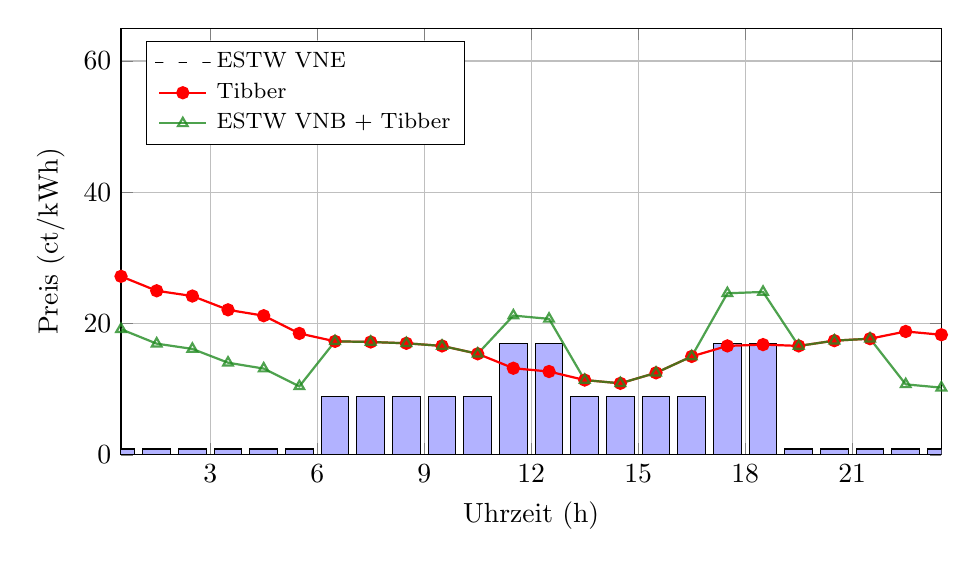
\begin{tikzpicture}
        \begin{axis}[
            width=12cm, height=7cm, % Größe des Plots
            xlabel={Uhrzeit (h)}, % Beschriftung X-Achse
            ylabel={Preis (ct/kWh)}, % Beschriftung Y-Achse
            xtick={0,3,6,9,12,15,18,21,24}, % Markierungen auf der X-Achse
            ymin=0, ymax=65, % Wertebereich für die Preise
            xticklabel style={anchor=north}, % Ausrichtung der X-Achsen-Beschriftung
            yticklabel style={anchor=east}, % Ausrichtung der Y-Achsen-Beschriftung
            grid=major, % Gitterlinien
            enlargelimits=false, % Begrenzung der Achsen direkt an den Rändern
            domain=0:24,
            legend pos=north west,
            legend style={font=\footnotesize},
            legend cell align=left
        ]
        
        % Beispiel: Balkendiagramm für stündliche Preise
        \pgfmathsetmacro{\vnt}{0.75*1.19}
        \pgfmathsetmacro{\vst}{7.52*1.19}
        \pgfmathsetmacro{\vht}{14.26*1.19}

        \addplot[ybar, fill=blue!30] coordinates {
            (0.5, \vnt) (1.5, \vnt) (2.5, \vnt) (3.5, \vnt) (4.5, \vnt) 
            (5.5, \vnt) (6.5, \vst) (7.5, \vst) (8.5, \vst) (9.5, \vst) 
            (10.5, \vst) (11.5, \vht) (12.5, \vht) (13.5, \vst) (14.5, \vst) 
            (15.5, \vst) (16.5, \vst) (17.5, \vht) (18.5, \vht) (19.5, \vnt) 
            (20.5, \vnt) (21.5, \vnt) (22.5, \vnt) (23.5, \vnt) 
        };
        \addlegendentry{ESTW VNE}
    
        % Alternative: Liniengrafik
        \addplot[thick, red, mark=*] coordinates {
            (0.5, 27.2) (1.5, 25) (2.5, 24.2) (3.5, 22.1) 
            (4.5, 21.2) (5.5, 18.5) (6.5, 17.3) (7.5, 17.2) 
            (8.5, 17) (9.5, 16.6) (10.5, 15.4) (11.5, 13.2) 
            (12.5, 12.7) (13.5, 11.4) (14.5, 10.9) (15.5, 12.5) 
            (16.5, 15) (17.5, 16.6) (18.5, 16.8) (19.5, 16.6) 
            (20.5, 17.4) (21.5, 17.7) (22.5, 18.8) (23.5, 18.3) 
        };
        \addlegendentry{Tibber}
        
        \pgfmathsetmacro{\vntsub}{\vst-\vnt}
        \pgfmathsetmacro{\vhtadd}{\vht-\vst}

        %NT:  0.75 ->  0.8925 (netto)
        %ST:  7.52 ->  9.9488 (netto)
        %HT: 14.26 -> 16.9694 (netto)
        \addplot[thick, ForestGreen, mark=triangle, opacity = 0.8] coordinates {
            (0.5, 27.2 - \vntsub) (1.5, 25 - \vntsub) 
            (2.5, 24.2 - \vntsub) (3.5, 22.1 - \vntsub) 
            (4.5, 21.2 - \vntsub) (5.5, 18.5 - \vntsub) 
            (6.5, 17.3) (7.5, 17.2) (8.5, 17) (9.5, 16.6) (10.5, 15.4) 
            (11.5, 13.2 + \vhtadd) (12.5, 12.7 + \vhtadd) 
            (13.5, 11.4) (14.5, 10.9) (15.5, 12.5) (16.5, 15) 
            (17.5, 16.6 + \vhtadd) (18.5, 16.8 + \vhtadd) 
            (19.5, 16.6) (20.5, 17.4) (21.5, 17.7) 
            (22.5, 18.8 - \vntsub) (23.5, 18.3 - \vntsub) 
        };
        \addlegendentry{ESTW VNB + Tibber}
        
        \end{axis}
    \end{tikzpicture}

\end{frame}

\begin{frame}{Beispielrechnungen (ESTW)}
    \begin{center}        
        \begin{tabular}{l c | S[table-format=2.2] c S[table-format=2.4]}
            \multicolumn{2}{c|}{\textbf{Tarif}} 
              & \multicolumn{1}{c}{\textbf{netto (ct/kWh)}} 
              & \multicolumn{1}{c}{} 
              & \multicolumn{1}{c}{\textbf{brutto (ct/kWh)}} \\\hline
            Niedertarif   & NT & 0.75  & → & 0.8925  \\
            Standardtarif & ST & 7.52  & → & 9.9488  \\
            Hochtarif     & HT & 14.26 & → & 16.9694
        \end{tabular}
           
    \end{center}

    % \begin{description}
    %     \item[WP] 10 kW\textsubscript{th}, 3 kW\textsubscript{el}: $\approx 9$ ct/h $\rightarrow$ 180 \EUR{}/a
    %     \item[Speicher] 10 kWh $\rightarrow$ $\approx 80$ ct/d, 200 d/a $\rightarrow$ 160 \EUR{}/a
    %     \item[E-Auto] 15 tkm, 60\%@\faHome, 17 kWh/100 km, $\approx 9$ ct/kWh $\rightarrow$ 140 \EUR{}/a
    % \end{description}

    \begin{tabular}{l l c l}
        \textbf{Was?} & \textbf{Annahmen} & \textbf{Einsparung} & \textbf{Jährlich} \\
        \hline
        WP       & \SI{10}{kW_{\text{th}}}, \SI{3}{kW_{\text{el}}}, 2000 h/a & $\approx$ 9 ct/h  & 180\EUR{}/a \\

        Speicher & \SI{10}{kWh}, 200 d/a & $\approx$ 80 ct/d & 160\EUR{}/a \\

        E-Auto   & \SI{15}{tkm}, 60\%@\faHome, \SI{17}{kWh/100km} & $\approx$ 9 ct/kWh  & 140\EUR{}/a \\
    \end{tabular}

    \begin{block}{Flexibilität als Schlüssel mit Einschränkungen}
        Durch Lastverschiebungen sind diese Einsprungen mit VNE gut erreichbar. Dynamische Strompreisen sind schlechter kalkulierbar und stark abhängig davon, wie gut und lange man die Last verschieben kann.
    \end{block}

\end{frame}
